\documentclass[12pt,a4]{article}

\usepackage{graphicx,subfigure,a4wide,noparindent}

\title{Designing complex Gabor filters}
\author{Bill Christmas}

\begin{document}

\maketitle

\section{Introduction}

In order to detect texture in scenes, the human visual system uses a set of bandpass filters that vary in orientation and centre frequency.  A Gabor filter bank is a set of regularly spaced filters that very approximately mimic this behaviour.  Typical filters might have point spread functions such as:

\begin{center}
  
\includegraphics{psf}  \hspace{2cm} 
\includegraphics{psf45}
\end{center}

\section{Design principles}

Consider first a single prototype filter, for example the left-hand example above.  Such a filter has a point spread function of the form:
\[ g(x,y) = {1 \over 2 \pi  \sigma_r\sigma_\theta}\;
\exp \left\{ -{1\over2} \left[{\left(x\over\sigma_r\right)^2+\left(y \over \sigma_\theta\right)^2}\right]\right\} \;
\cos\left(2\pi U x\right) \]
The exponential term defines a Gaussian-shaped envelope of elliptical shape, and the cosine term defines the centre frequency.  The Gaussian envelope shape is used to get the best compromise of minimising the filter width in both spatial and frequency domains.  The constants are chosen so that the filter has unity gain at zero frequency, with parameters $\sigma_r, \sigma_\theta$ that express the filter width as a ``standard deviation'' in units of pixels.

The problem with such a p.s.f.\ is that the response ripples in a similar manner to the cosine term in the p.s.f.  A convenient way to deal with this is instead to use a complex p.s.f.:
\[ g(x,y) = {1 \over 2 \pi  \sigma_r\sigma_\theta}\;
\exp \left\{ -{1\over2} \left[{\left(x\over\sigma_r\right)^2+\left(y \over \sigma_\theta\right)^2}\right]\right\} \;
\exp\left(i2\pi U x\right) \]
and to deal with the resulting complex filtered image by taking its modulus.  This gives a final response whose shape is influence by the Gaussian envelope of the p.s.f.\ instead of the p.s.f.\ itself.

The Fourier transform of the p.s.f.\ is given by:
\begin{equation}
  G(u,v) = \exp \left\{ -2\pi^2\left[ \sigma_r^2 (u-U)^2 +\sigma_\theta^2 v^2 \right] \right\}\label{eq:G}
\end{equation}
--- i.e.\ an elliptical shape whose centre is offset on the $u$ axis by the centre frequency $U$.

The frequency coordinate system can then be rotated and scaled to create an array of filters of $N$ different orientations and $M$ different scales, using the substitution:

\[ {u \choose v} = s^m \left( \begin{array}{rr}\cos \pi{n\over N} & \sin
    \pi{n\over N} \\ -\sin \pi{n\over N} & \cos \pi{n\over N}
  \end{array}\right) {u' \choose v'} ,\; m = 0, 1, \ldots, M-1,\; n = 0, 1,
\ldots N-1,\; s > 1 \] where $u', v'$ are the coordinates of a general filter.
The scale ratio parameter $s$ thus defines both the ratio of the centre
frequencies of filters of adjacent scales, and also their widths.

If we are using these filters for digital image processing, we also need to determine the frequency scales, to ensure that the same proportion of the spectrum is covered in both dimensions.  In the above analysis, the frequencies $u, v$ are in the continuous domain, and have units of cycles per unit length.  We can arbitrarily choose our unit length to be a pixel width, $p$ (assuming square pixels), in which case the frequency units are $1/p$.  In the sampled domain however the frequency units are related to the image dimensions (which are generally different from each other).  If the image width and height are $L_w$ and $L_h$ pixels respectively, the units of the frequency samples are $1/(L_w p)$, $(1/L_h p)$.  Hence if the sampled frequencies are $k_u, k_v$, then
\[ {u' \choose v'} = {{k_u \over L_w} \choose {k_v \over L_h}} \]

The result is a set of filters that covers one half of the complex frequency plane, shown in Fig.~\ref{fig:spectrum}.  (We do not populate the lower half of the plane because the extra filters would have the same response as the existing ones.)  The set of filters can be made a little more compact by offsetting every other scale by $1\over 2$ of the angular separation, shown in Fig.~\ref{fig:shifted} (here the middle of the 3 scales).  Note however that this will reduce the number of filters that explicitly detect perceptually important vertical lines.
\begin{figure}[t]\centering
  \subfigure[no offset]{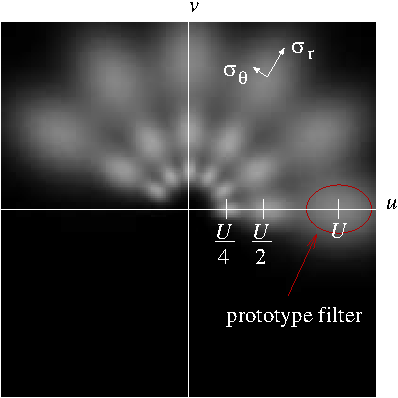
\includegraphics{maskfig}\label{fig:spectrum}}
  \hspace{2em}
  \subfigure[with alternate scales offset]{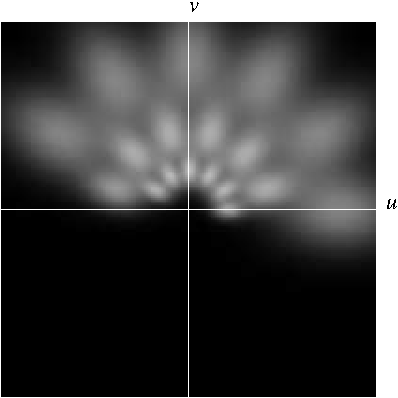
\includegraphics{offsetfig}\label{fig:shifted}}
  \caption{Spectral representation of filters: $M=3$, $N=6$, $s=2$\label{fig:spectra}}
\end{figure}

\section{Setting the scale parameters}


The filter scale parameters are set as follows.  Note that $\sigma_\theta$, $\sigma_r$ are the filter scales in the {\em spatial} domain.  

\paragraph{$\mathbf{\sigma_\theta}$:} 
This represents the filter scale in pixels in the tangential direction of the highest frequency filters.  It is more or less inversely proportional to the tangential filter separation.  Half-way between the centres of two filters adjacent in the tangential direction, the filter responses are equal ($=\delta$, say where $\delta < 1$). The distance between the two filters is given by (Fig.~\ref{fig:circles}):
\def\Sinpbnn{\sin{\left(\pi\over2N\right)}}
\[ 2r = 2U \Sinpbnn \]
Since  $\delta$ is the response of a filter at a distance $U\sin(\pi/2N)$ from its centre in what is approximately the tangential direction, and $u$ is constant in the tangential direction ($u = U$ for the highest frequency filters), then from (\ref{eq:G}):

\[ \delta = \exp \left[ -2\pi^2 \left(\sigma_\theta U \Sinpbnn\right)^2  \right] \]
\[ \rightarrow\quad \sigma_\theta =
  \sqrt{-\ln\delta \over 2\pi^2}\; {1 \over U\Sinpbnn} 
\]

Using $\delta = {1\over2}$ gives a reasonably uniform overall coverage of the spectrum in the tangential direction, in which case:
\[ \sigma_\theta \approx {0.19 \over U\Sinpbnn} \]

\paragraph{$\mathbf{\sigma_r}$, no offsetting:}
$\sigma_r$ represents the filter scale in the radial direction of the highest frequency filters (the outer semi-ring in Fig.~\ref{fig:spectra}).  If we do not offset alternate scales (Fig.~\ref{fig:spectrum}), $\sigma_r$ and $\sigma_\theta$ are independent, so $\sigma_r$ depends only on the radial filter separation, which is a function of the scale ratio $s$.  The responses $\delta$ of the two outermost radially adjacent filters are equal when
\[ \exp\left[ -2\pi^2 \sigma_r^2 (u-U)^2\right]
= \exp\left[ -2\pi^2 \sigma_r^2 \left(su-U\right)^2\right] = \delta \]

Selecting appropriate roots:
\begin{eqnarray}
   \sigma_r &=& \sqrt{-\ln{\delta}\over 2\pi^2} \;{s+1\over U(s-1)} \label{eq:sigma_r}\\
   &=& {s+1\over s-1}\; \Sinpbnn\; \sigma_\theta \nonumber
\end{eqnarray}
For $\delta={1\over2}$:
\[ \sigma_r \approx 0.19 {s+1\over U(s-1)} \]
 
\paragraph{$\mathbf{\sigma_r}$, with offsetting:}
When alternate scales are offset by one half of the filter width (Fig.~\ref{fig:shifted}) the situation is more complicated.  Consider first the case when the filters are circular, i.e.\ 
\begin{equation}
  \label{eq:circ}
  \sigma_r = \sigma_\theta
\end{equation}

\begin{figure}
  \centering
  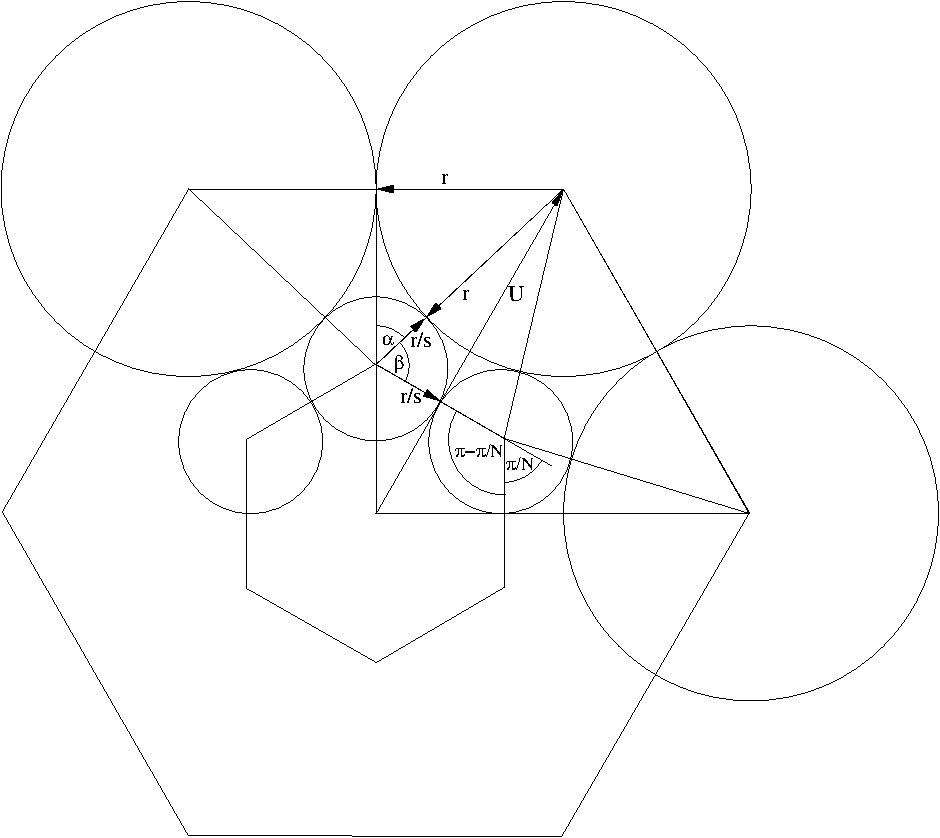
\includegraphics[width=0.6\textwidth]{circles}
  \caption{Geometry for offset circular Gabor filters; $N = 3$}
  \label{fig:circles}
\end{figure}
From basic geometrical properties (Fig.~\ref{fig:circles}), we can see that 
\[ \alpha + \beta = {N+1\over 2N}\pi, \quad \sin\alpha = {s_c\over 1+s_c}, \quad \cos\beta = {1\over 1+s_c} \]
where $N$ is the number of filters at the same scale, and $s=s_c$ is the scale ratio required to generate circular filters.

Defining $\tau = \sin\left({N+1\over 2N}\right)$, we can solve for $s_c$:
\[ s_c = {1+\tau-\tau^2 \pm \sqrt{(1+2\tau)(1-\tau^2)}\over \tau^2} \]
The positive root is the required one; the negative one corresponds to $1\over s$. For $N=4$, $s \approx 2$.

In the general case, for a desired value of $s$ we can use (\ref{eq:sigma_r}), (\ref{eq:circ}) to determine an appropriate value for $\sigma_r$:
\[ \sigma_r = {s+1 \over s-1}\: {s_c-1 \over s_c+1}\: \sigma_\theta \]


\section{Speeding up the filtering}

A common complaint of Gabor filters is that the inverse FFT that has to be performed for each of the filters makes the system too slow to be useful.   The basic method performs a 2D inverse FFT over the whole filtered image spectrum.  However, most of this spectrum has almost no energy for a given filter.  If instead we shift the coordinates of the spectrum to the centre frequency of the filter, and crop this spectrum so that we only include regions where the filter has a significant response, the FFT will be correspondingly smaller and hence faster.  Because of the shift of frequency coordinates, the output image is multiplied by a phase term.  Since we take the modulus of the output image, this phase term is removed.  The output image is also smaller: it is the same size as the cropped spectrum.  However, if needed, it can be reinterpolated up to the original image size.  

\end{document}


